    The CAM-SE 
 uses   cubed-sphere geometry  originally introduced by \cite{S1972MWR}  to represent the planet earth. The  spherical   surface 
  $\mathcal{S}$ is  a patched domain,  which is partitioned  into   non-overlapping quadrilateral elements 
 $\Omega_e$ such that $\mathcal{S} = \cup \, \Omega_e$ (see Fig.~\ref{fig:gll4}). 
  On   $\mathcal{S}$  each 2D  element $\Omega_e(x^1,x^2)$  defined in terms of
 central  (gnomonic) projection angles $x^1,x^2 \in [-\pi/4, \pi/4]$, which serve as  the independent variables in the computational domain. 
 The mapping from cube to sphere results in a non-orthogonal curvilinear  coordinate system on $\mathcal{S}$, with 
 the  metric tensor $G_{ij}$ and  analytic Jacobian $ \sqrt{G} =  |G_{ij}|^{1/2}$, $i, j \in \{1,2\}$. 
 A  physical vector quantity  such as the wind vector $\mathbf{v} = (u,v)$,  defined on  $\mathcal{S}$
 in  orthogonal lat-long coordinates,  can  be uniquely
 expressed in tensor form using conventional notations as the covariant $(u_1,u_2)$ and contravariant  $(u^1, u^2)$ vectors 
 using the  $2 \times 2$ transformation matrix  $\mathbf{D}$ associated with the gnomonic mapping 
 such that   $\mathbf{D}^T\mathbf{D} = G_{ij}$ (see \cite{NTL2005MWR} for the details):  
  %   
    \begin{equation}
     \left[   \begin{array}{c}
               u \\ v
             \end{array}
           \right]
           =
     \mathbf{D}  \, \left[   \begin{array}{c}
               u^1 \\ u^2
             \end{array}
           \right] =
            \mathbf{D}^{-T}  \, \left[   \begin{array}{c}
               u_1 \\ u_2
             \end{array}
           \right]. 
%          \quad \mathbf{D}^T\mathbf{D} = G_{ij}. 
          \label{eq:covcontra} 
\end{equation}

 The governing equations defined in familiar vector form can also be expressed 
 in  general tensor form. In order  to  describe the SE discretization process in simple terms, we consider the 
 the following conservation law  on $\mathcal{S}$ for an arbitrary  scalar $\phi$:  
 %
 \begin{equation}
 \frac{\partial \phi }{\partial t}  + \nabla \cdot \mathbf{F}(\phi)  = S(\phi)   \quad   
 \Rightarrow   %\frac{\partial U }{\partial t}  + \nabla_h \cdot \mathbf{F}(U)  = S(U), 
   \frac{\partial \phi }{\partial t}  + \frac{1}{\sqrt{G}} \left[   \frac{\partial  \sqrt{G} F^1}{\partial x^1}  + 
   \frac{\partial  \sqrt{G} F^2}{\partial x^2}      \right]   = S(\phi),  
  \label{eq:se1} 
   \end{equation} 
  %
  where  equation of the right side is a special case, the flux-form transport equation, with 
   contravariant fluxes $(F^1, F^2) = (u^1 \phi , u^2 \phi)$, and $S(\phi)$  is an arbitrary source term.
%  and  the gradient $\nabla_h = (\partial/\partial x^1, \partial/\partial x^2)$ defined on computational domain $\mathcal{C}$ corresponding
%  to $\mathcal{S}$ under the gnomonic mapping.   Note that the flux-form  transport  equation  is a special case of (\ref{eq:se1}), with flux function
%  $(F^1, F^2) = (u^1 U,  u^2 U)$.

  
\subsection{\normalsize SE spatial discretization in 2D}

%In order to describe the spectral-element (SE) horizontal discretization as used in CAM-SE, we consider the
%following generic form  of a governing equation (33-35): 
% \begin{equation}
% \frac{\partial U }{\partial t}  + \nabla_h \cdot \mathbf{F}(U)  = S(U)   \quad   {\rm in} \quad \mathcal{S}, \label{eq:se1} 
% \end{equation} 
% %
%where $U$ is a prognostic variable defined on the spherical domain $\mathcal{S}$ and  $\nabla_h \cdot$ is the horizontal divergence operator. 
%$\mathbf{F}$ is a general  flux function and $S(U)$ is the source term, which can be
%a diffusive flux or any forcing term.  

The  SE solution process involves  casting the PDE in Galerkin form, i.e.,  by multiplying  (\ref{eq:se1})  with a test (weight) function
$\psi$  and integrating over the domain $\mathcal{S}$, 
\begin{equation}
 \int_{\mathcal{S}} \psi \,  \left[ \frac{\partial \phi }{\partial t}  + \nabla \cdot \mathbf{F}(\phi) -  S(\phi)  \right]  d\mathcal{S}  = 0. \label{eq:se2} 
 \end{equation} 
A computational form of  (\ref{eq:se2})  is obtained by applying Green's theorem,  
resulting in  the weak Galerkin form as follows: 
 %
 \begin{equation}
 \int_{\mathcal{S}} \psi   \ \frac{\partial \phi }{\partial t} \,   d\mathcal{S}  = 
  \int_{\mathcal{S}}  \nabla  \psi \cdot \mathbf{F}(\phi) \,  d\mathcal{S}  + 
       \int_{\mathcal{S}} \psi  \, S(\phi)  \,   d\mathcal{S}, \label{eq:se3} 
 \end{equation} 
 %
 where the approximation to the  solution $\phi$ and the test function belong to a polynomial space  $V^{N}$. 
 The SE method consists of  partitioning the domain into non-overlapping elements and solving the global problem 
 locally on each element, where the  solution is approximated by using a set of  basis (polynomial) functions of prescribed 
 order $N$.  A basic assumption used in SE (or continuous Galerkin) method is that the global basis 
 corresponding to (\ref{eq:se3}) is 
 $C^0$ continuous. 
Therefore  the problem (\ref{eq:se3}) can be solved locally for each 
 element $\Omega_e$, if there is a mechanism by which the solution maintains $C^0$ 
 continuity at the element boundaries as required 
 by the SE  discretization.   
 %
  \begin{figure}[h]
\centering
 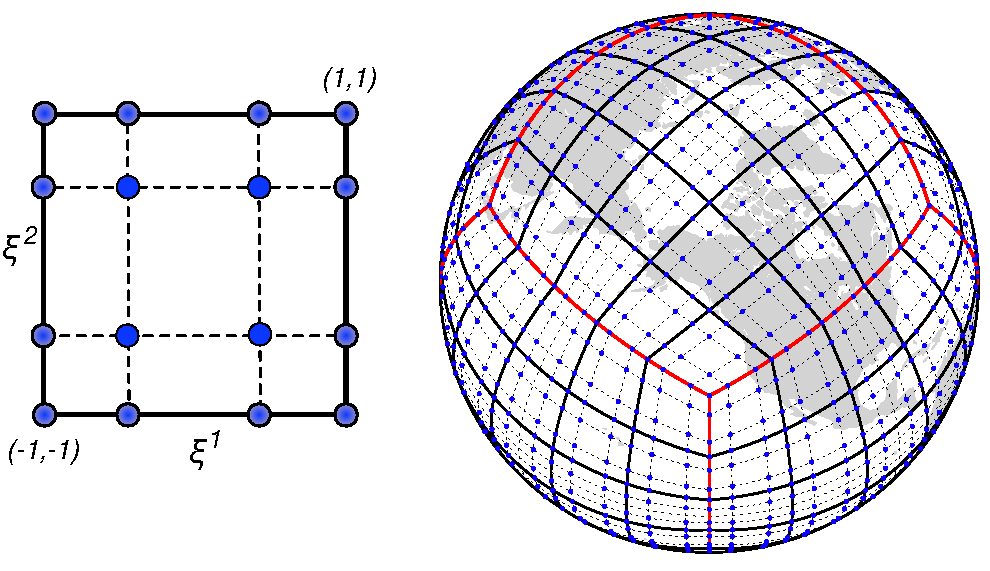
\includegraphics[scale=0.75]{figs/cs_gll4_2017}
 \caption{The left panel shows the  Gauss-Lobatto-Legendre (GLL)   grid with $ N_p \times  N_p$ quadrature points defined
 on a standard element $[-1,1]^2$, where $N_p=4$. The right panel shows the cubed-sphere ($\mathcal{S}$) grid system tiled with 
 $6 N_e^2 $ spectral elements $\Omega_e$, where $N_e$ is the number of elements  in each coordinate direction
 on a panel. 
 Each element  $\Omega_e$ on $\mathcal{S}$ has the GLL grid structure.  }
 \label{fig:gll4}
\end{figure}
%
 
 For efficient evaluation of the integral equation (\ref{eq:se3}), the SE  method employs the Gauss-Lobatto-Legendre (GLL) 
  quadrature rule for integrals and collocation differentiation for derivative operators. All the corresponding numerical 
  operations are performed on a square   $[-1,1]^2$ known as  the standard  (or reference) element.   
%  For that each 2D  element $\Omega_e(x^1,x^2)$  defined in terms of
% central angles $x^1,x^2 \in [-\pi/4, \pi/4]$, which are  essentially the independent variables 
% in the physical domain (Nair et al. 2004).  
 In order to facilitate local mesh refinement,   
  the spectral elements  $\Omega_e$  on $\mathcal{S}$ are defined as arbitrary spherical quadrilaterals
  in  the CAM-SE  grid system, which should   be  mapped onto  the standard element.
  A direct  way to address this problem is establishing  % a composite mapping  in computational space. 
  a  transformation  $\mathcal{J}_e: \Omega_e \rightarrow [-1,1]^2$, where    $\mathcal{J}_e$
  may be considered as   a  composite mapping combining the gnomonic and  the quadrilateral to standard-element mapping.
  Let the Jacobian  associated  with the composite mapping be $J_e = J_e(\sqrt{G})$.
   Then   an  arbitrary surface integral  on $\Omega_e$ can be expressed in terms of local coordinates $\xi^1, \xi^2 \in [-1, 1] $
 and the Jacobian  $J_e$; 
   %
   \begin{equation}
 \int_{\Omega_e} \psi (x^1,x^2) \,  d\Omega_e =   \int_{-1}^{1} \int_{-1}^{1} J_e(\xi^1,\xi^2)  \,  \psi(\xi^1,\xi^2) \, d\xi^1 \, d\xi^2
   \approx   \sum_{k=0}^{N}   \sum_{l=0}^{N} w_k w_l \, J_e(\xi^1_k,\xi^2_l) \,   \psi(\xi^1_k,\xi^2_l),
                               \label{eq:se4} 
 \end{equation} 
 %
 where  $w_k, w_l$  are  the  Gauss  quadrature weights. 
 
 In the  case of GLL quadrature rule, the  nodal points $\xi_k$, $k=0, 1, \dots, N$, 
 are  the roots of  the polynomial $(1-\xi^2) P'_N(\xi) = 0$,
 $\xi \in [-1,1]$;   and the corresponding  GLL quadrature  weights are given by 
 \[   w_k =  \frac{2}{N(N+1) \, [P_N(\xi_k)]^2 },
 \] 
  where  $P_N(\xi)$ is the  Legendre polynomial of degree $N$. 
   For the SE discretization it is customary to use  Lagrange polynomials  $h_k(\xi)$,   with roots at  the 
 GLL   quadrature points $\xi_k$, as basis functions.  This setup provides  discrete orthogonality 
 for  the basis function $h_k(\xi)$,  which   is formally defined as: 
 %
 \begin{equation}
    h_k(\xi) = \frac{ (\xi^2-1)\, P'_N(\xi)}{ N (N+1)\, P_N(\xi_k) \,(\xi-\xi_k)}.   \label{eq:se5}
 \end{equation}
 %
  Note that there are $N+1 = N_p$ GLL quadrature points in 1D,
 and $N_p \times N_p$ GLL points are needed for 2D spectral elements $\Omega_e$. 
 Figure~(\ref{fig:gll4}) shows the GLL grid  with $N_p =4$ on the left panel, 
 and the right panel shows the cubed-sphere grid $\mathcal{S}$ tiled with elements $\Omega_e$,
 each with the GLL  grid points. 
 
  A semi-discrete  form of  (\ref{eq:se3})  on an  element $\Omega_e$ can by obtained by
   approximating the solution  as a tensor product of  1D Lagrange basis  $\{ h_k(\xi)\}_{k=0}^N$ such that
  %
 \begin{equation}
     \phi |_{\Omega_e} \approx  \phi^e(\xi^1,\xi^2,t) =  
              \sum_{k=0}^{N}   \sum_{l=0}^{N}  \phi^e_{kl}(t)  \, h_k(\xi^1) \, h_l(\xi^2),  \label{eq:se60}
 \end{equation}
 %
 where $\phi^e_{kl}(t) = \phi^e(\xi_k^1, \xi_l^2,t) $ are  the nodal grid-point values of the solution, and  defining the  test function as
  $\psi(\xi^1,\xi^2) = h_k(\xi^1) \, h_l(\xi^2)$. By using (\ref{eq:se4}) and discrete orthogonality property of $h_k(\xi)$, 
  we get a completely decoupled system of ODEs on  $\Omega_e$,  for each grid-point $(k,l)$  we have 
  %
  \begin{eqnarray}
      M^e_{kl}\, \, \frac{d }{dt} \phi^e_{kl}(t) &= &  A^e_{kl}    + S^e_{kl}  \label{eq:se6} \\
        M^e_{kl}  &=  & \int_{-1}^{1} \int_{-1}^{1} J_e  \, h_k(\xi^1)  \, h_l(\xi^2) \, d\xi^1  d\xi^2 = J_e(k,l) \, w_k \, w_l \\
          A^e_{kl}  &=  & \sum_{i=0}^N  J^{(1)}_e(i,l) \,  F^1_{i l} \, D_{ik}^{(1)}\, w_i  w_l  +
           \sum_{i=0}^N  J^{(2)}_e(k, i) \,  F^2_{k i} \, D_{l i}^{(2)} \, w_k  w_i \\
           S^e_{kl}  &=   &J_e(k,l) \, w_k w_l  \, S(U_{kl})
  \end{eqnarray}  
  %
  %where $  M^e_{kl}$ is the so-called  mass matrix, $(F^1,F^2) = \mathbf{F}$  are  the  flux terms, 
   where $J^{(i)}_e = J_e \,\partial \xi^i / \partial x^i$ is the metric term  and 
   $D^{(i)}_{lk}$ is the  derivative matrix $h'_k(\xi^i_l)$, 
  along $x^i$-direction and  $ i \in \{1,  2\}$.  The ODEs  (\ref{eq:se6}) can be written a formal matrix-vector form
  for  $\Omega_e$  as follows:
  \cite{KS2013book}: 
  %
 \begin{equation}
    \mathbf{M}^e\, \, \frac{d }{dt} \Phi^e =   \mathbf{A}^e    + \mathbf{S}^e + \mathbf{B}^e,  \label{eq:se7} 
 \end{equation}
      %
      where $\mathbf{M}^e$ is the  so-called mass matrix,  which  is a diagonal  matrix with entries $M^e_{kl}$.    $\mathbf{B}^e$
  indicates the boundary terms for the element 
  $\Omega_e$, which is a key component linking  the local and global problem (\ref{eq:se3}) and enforcing $C^0$ continuity
  for solutions across element boundaries.  
  
  The  global matrices associated with  (\ref{eq:se3}) can be obtained 
  by  summing the contributions from elemental matrices  and  this procedure is known as the 
  direct stiffness summation (DSS). However the global matrices are  not explicitly constructed. 
  In practice, the DSS operation replaces  interface values  of two  contiguous elements sharing the same physical location  
  by the  weighted sum (average)  so that  the boundary  nodes get unique values,   
   which maintains the continuity of the global solution across the element edges. This strategy has been adopted in CAM-SE. 
  Note that the DSS operation does not affect interior nodal values of any element, and  preserves global conservation of SE discretization
  for (\ref{eq:se1}).  The elemental discretization (\ref{eq:se7}) combined with the  DSS operation  ($ \mathcal{L}_h$) leads 
  to the time-dependent  system of ODE corresponding to (\ref{eq:se1}),
     \begin{equation}
  \frac{d }{dt} \phi(t) =   \mathcal{L}_h(\phi).  \label{eq:se8}
       \end{equation}

   
   \subsection{Dissipation}\label{sec:dissipation}
   In the CAM-SE model explicit  fourth-order hyperviscosity  ($\nu \nabla^4 \phi$) used as 
    the main stabilization mechanism.  For scalar fields such as $T, p, q$ etc., 
   a scalar viscosity   is applied,  while  for the horizontal momentum equations vector viscosity
   ($\nu \nabla^4 \mathbf{v} $) is employed. The coefficient of viscosity $\nu$ may be constant or a spatially varying 
  quantity  depending on the application. High-order viscosity operator $ \nu \nabla^{2m} \phi$, $m=2,3, \dots$, 
    for an arbitrary variable $\phi$  can be constructed 
  by successively applying the basic Laplacian-type viscosity operator $\nabla^2 ( \,)$. In order to describe the SE discretization 
  we consider the basic Laplacian without the coefficient of viscosity $\nu$: 
   \begin{equation}
   L(\phi)  = \nabla^2 \phi .  \label{eq:Laplace}
   \end{equation}
   %
  Integrating  (\ref{eq:Laplace}) over an element $\Omega_e$  with boundary $\Gamma_e$, using Greens method   results in 
    \begin{equation}
  %
  \int_{\Omega_e}  L \, \psi  \,  d \Omega_e  =   \int_{\Gamma_e}  \phi \nabla \psi  \,    d  \Gamma_e - 
                      \int_{\Omega_e}  \nabla \psi \cdot \nabla \phi \,  d \Omega_e  \label{eq:Lweak}
   \end{equation}
   For the continuous Galekin (SE) method the boundary integral vanishes ($\psi = 0$ at the element boundaries) 
   and the  {\em  rhs} simplifies to 
   a surface integral.   The tensor gradients in the integrand  can be expressed  in terms of its contravariant  components 
   $(\tilde{F}^1, \tilde{F}^2)$, using (\ref{eq:covcontra}) such that 
 \begin{equation}
    \nabla \psi \cdot \nabla \phi  = \tilde{F}^1  \frac{\partial \psi}{ \partial x^1} +
      \tilde{F}^2  \frac{\partial \psi}{ \partial x^2} , \quad 
  %
    % 
     \left[   \begin{array}{c}
               \tilde{F}^1  \\     \tilde{F}^2
             \end{array}
           \right]
           =
     \mathbf{D}^{-1}  \mathbf{D}^{-T}   \, \left[   \begin{array}{c}
                \partial \phi / \partial x^1  \\ \partial \phi / \partial x^2 
             \end{array}
           \right] 
           \label{eq:Tgrad}.
  \end{equation}
Thus the discretization of the Laplacian for SE method can be obtained by simplifying the integral 
%
 \begin{equation}
   \int_{\Omega_e}  L \, \psi  \,  d \Omega_e  = -   \int_{\Omega_e}  \nabla \psi \cdot \nabla \phi \,  d \Omega_e
    = -  \int_{\Omega_e} \left[  \tilde{F}^1  \frac{\partial \psi}{ \partial x^1} +
      \tilde{F}^2  \frac{\partial \psi}{ \partial x^2}  \right]    d \Omega_e.  \label{eq:Lap0}
  \end{equation}
  %
 As in the case of  (\ref{eq:se6}),  the weak formulation (\ref{eq:Lap0})  can be evaluated  on the standard element   
  using    the polynomial approximations (\ref{eq:se60}) for $\phi, \psi$ on $\Omega_e$ and GLL quadrature rule.
   Further simplification of (\ref{eq:Lap0})  leads to 
 %
   \begin{equation}
     L^e_{kl} =  - ( M^e_{kl})^{-1} \left[ 
           \sum_{i=0}^N  J^{(1)}_e(i,l) \,  \tilde{F}^1_{i l} \, D_{ik}^{(1)}\, w_i  w_l  +
           \sum_{i=0}^N  J^{(2)}_e(k, i) \,  \tilde{F}^2_{k i} \, D_{l i}^{(2)} \, w_k  w_i  \right], 
           \label{eq:Lap1}
   \end{equation}
 where $L^e_{kl}$ is the value of Laplacian term for a gridpoint $(k,l)$ on $\Omega_e$.  
 
 
   Note that in practice,
 the contravariant gradient terms in  (\ref{eq:Tgrad}) are fist  computed using collocation differentiation,   
 then  the weak  divergence of the gradients   is computed;    this is followed by a  DSS operation which 
 yields the discrete Laplacian ($ L(\phi^e)  \Rightarrow  div(grad(\phi^e))$). 
 
 In CAM-SE the vector viscosity is handled  using the vector Laplacian $\nu \nabla^2 \mathbf{v}$, 
 which is consistent with the curvilinear formulation of the momentum equation.  By using the vector identity 
 $\nabla^2 \mathbf{v} = \nabla(\nabla \cdot \mathbf{v}) - \nabla \times (\nabla \times \mathbf{v}) $, 
 the coefficient of viscosity $\nu$ may be split into the viscosity corresponding to the divergence part $\nu_d$
 and that for  the vorticity part $\nu_v$ such that 
 %
 \begin{equation}
  \nu \nabla^2 \mathbf{v} = \nu_d \, \nabla(\nabla \cdot \mathbf{v}) -
   \nu_v \,  \nabla \times (\nabla \times \mathbf{v}). \label{eq:vLap}
 \end{equation}
   %
   The SE discretization  of (\ref{eq:vLap}) is handled separately for each component using a vector test function
   $\vec{ \psi}$ and the weak formulation: 
   %
   \begin{eqnarray}
       \nu_d  \int_{\Omega_e} \vec{\psi} \cdot   \nabla(\nabla \cdot \mathbf{v})  \,    d \Omega_e  & = & 
       -  \nu_d \, \int_{\Omega_e} (\nabla \cdot \vec{\psi})   (\nabla \cdot \mathbf{v})   d \Omega_e \\
         -   \nu_v  \int_{\Omega_e}     \vec{\psi} \cdot  \nabla \times (\nabla \times \mathbf{v})   \,    d \Omega_e  & = &
                          -   \nu_v  \int_{\Omega_e} (\nabla \times      \vec{\psi} ) \cdot (\nabla \times \mathbf{v})    \,     d \Omega_e ,  
   \end{eqnarray}
   where the line integrals along the boundaries associated with weak formulation  vanishes for SE discretization. 
   The {\em rhs} of the above equations are converted into equivalent tensor form  for the divergence and curl terms,
   and discretized as in the case of (\ref{eq:Lap1}). 
   
 





